\subsection{Algorytm mediana median}
Algorytm wygląda następująco:
\begin{verbatim}
findK(S, k);
    if |S| < 50 then
        sort(S);
        return S[k];
    S1, S2, ... Sn/5 = split(S) // podziel S na 5-elementowe podzbiory;
    sort(S1); ... sort(Sn/5);
    Q = {median(S1), ..., median(Sn/5)}
    m = findK(Q, n/10)
    S1 = {x in S: x < M};
    S2 = {x in S: x = M};
    S3 = {x in S: x > M};
    if (|S1| ≥ k)
        return select(S1, k);
    if (|S1| + |S2| ≥ k)
        return M;
    return select(S3, k-|S1|-|S2|);
\end{verbatim}


\subsection{Złożoność}
Kluczową obserwacją jest, że \( \abs{S_1}, \abs{S_3} \leq \frac{3}{4}n \).
Posortowane 5-elementowe podzbiory można przedstawić jak na rysunku poniżej:
\begin{figure}[H]
    \centering
    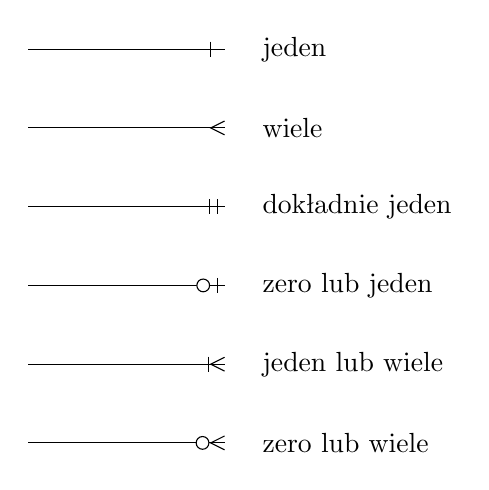
\begin{tikzpicture}
\usetikzlibrary{arrows.meta}

\pgfdeclarearrow{name = No Tip, drawing code=}
\tikzset{
  ER tip sizes/.style n args={3}{
    ER Bar/.tip     ={Bar[width={#2 +1}]},
    ER Circle/.tip  ={Circle[fill={#3}, width={#2}, length={#1}]},
    ER One/.tip     ={ER Bar[sep={#1}] No Tip[]},
    ER Many/.tip    ={Straight Barb[reversed, width={#2}, length={#1}] No Tip[]},
    ER OneOnly/.tip ={ER Bar[sep={(#1)/2}] ER Bar[sep={(#1)/2}] No Tip[]},
    ER ZeroOne/.tip ={ER Circle[sep={(#1)/2}] ER Bar[sep={(#1)/2}] No Tip[]},
    ER OneMany/.tip ={ER Bar[] ER Many[]},
    ER ZeroMany/.tip={ER Circle[] ER Many[]}
  },
  ER tip sizes={+5pt}{+5pt}{white}
}

\draw[arrows=-ER One]      (0,-1) -- ++(right:2.5) node[right]{\quad jeden};
\draw[arrows=-ER Many]     (0,-2) -- ++(right:2.5) node[right]{\quad wiele};
\draw[arrows=-ER OneOnly]  (0,-3) -- ++(right:2.5) node[right]{\quad dokładnie jeden};
\draw[arrows=-ER ZeroOne]  (0,-4) -- ++(right:2.5) node[right]{\quad zero lub jeden};
\draw[arrows=-ER OneMany]  (0,-5) -- ++(right:2.5) node[right]{\quad jeden lub wiele};
\draw[arrows=-ER ZeroMany] (0,-6) -- ++(right:2.5) node[right]{\quad zero lub wiele};
\end{tikzpicture}
\end{figure}
Elementy prawej dolnej ćwiartki są nie mniejsze niż \( m \), więc \( S_1 \) musi zawierać się w pozostałych trzech ćwiartkach. 
Analogicznie elementy lewej górnej ćwiartki są nie większe niż \( m \), więc \( S_4 \) również musi mieścić się w trzech ćwiartkach. 

Złożoność algorytmu jest opisana równaniem:
\[ T(n) \leq c, dla n < 50 \]
\[ T(n) \leq T(n/5) + T(3/4 n) + c \cdot n,\; n \geq 50 \]
Można pokazać indukcyjnie, że \( T(n) \leq 20 \cdot c \cdot n = \Theta(n) \).

Wynika to również z twierdzenia: \\
Jeśli \( c_i > 0, i = 1, \dots, m, \sum_{i=1, \dots, m} c_i < 1 \), to rozwiązanie
równania
\[ T(n) =\sum_{i=1, \dots, m} T(c_i \cdot n) + \Theta(n) \]
spełnia \( T(n) = \Theta(n) \).

Dlaczego magiczne piątki? \\
Dla trójek równanie rekurencyjne jest postaci
\[ T(n) = T(n/3) + T(2n/3) + O(n), \]
a \( \frac{1}{3} + \frac{2}{3} \not< 1 \) i jego rozwiązaniem jest \( T(n) = \Theta(n \log n) \).
Jeśli chodzi o siódemki, złożoność jest taka sama jak w przypadku piątek, jednak posortowanie zbiorów 7-elementowych wymaga niewątpliwie większej liczby porównań niż zbiorów 5-cio elementowych.
Ot i cała magia